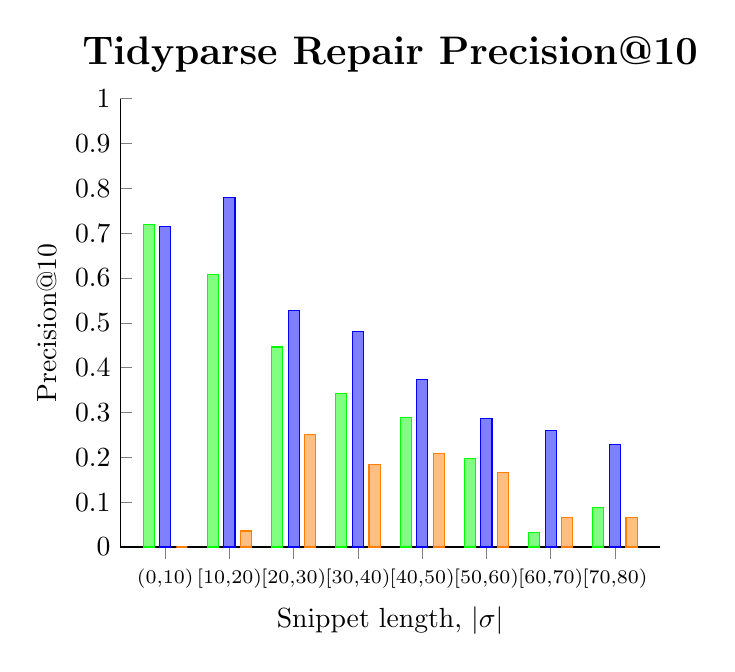
\begin{tikzpicture}
  \begin{axis}[
  xlabel={Snippet length, $|\sigma|$},
  ylabel={Precision@10},
  title={\Large\textbf{Tidyparse Repair Precision@10}},
  ybar,
  axis lines*=left,
  xtick={0, 10, 20, 30, 40, 50, 60, 70},
  ytick={0, 0.1, 0.2, 0.3, 0.4, 0.5, 0.6, 0.7, 0.8, 0.9, 1.0},
  xticklabels={{(}0{,}10{)}, {[}10{,}20{)}, {[}20{,}30{)}, {[}30{,}40{)}, {[}40{,}50{)}, {[}50{,}60{)}, {[}60{,}70{)}, {[}70{,}80{)}},
  x tick label style={font=\scriptsize},
  ymax=1.0,
  ymin=0.0,
  bar width=4pt,
  ]
  \addplot[green, fill=green!50] coordinates { (0, 0.71875) (10, 0.6075268817204301) (20, 0.44621513944223107) (30, 0.3427230046948357) (40, 0.288) (50, 0.19791666666666666) (60, 0.03333333333333333) (70, 0.08823529411764706) };
  \addplot[blue, fill=blue!50] coordinates { (0, 0.7142857142857143) (10, 0.7789473684210526) (20, 0.5277777777777778) (30, 0.4803921568627451) (40, 0.37333333333333335) (50, 0.2857142857142857) (60, 0.26) (70, 0.22857142857142856) };
  \addplot[orange, fill=orange!50] coordinates { (0, 0.0) (10, 0.03571428571428571) (20, 0.25) (30, 0.18421052631578946) (40, 0.20833333333333334) (50, 0.16666666666666666) (60, 0.06666666666666667) (70, 0.06666666666666667) };
  \end{axis}
\end{tikzpicture}